\testfile{pgfplotstest.expr.tex}
\testsection{`plot expression' test}
\testsubsection{sin(x)}
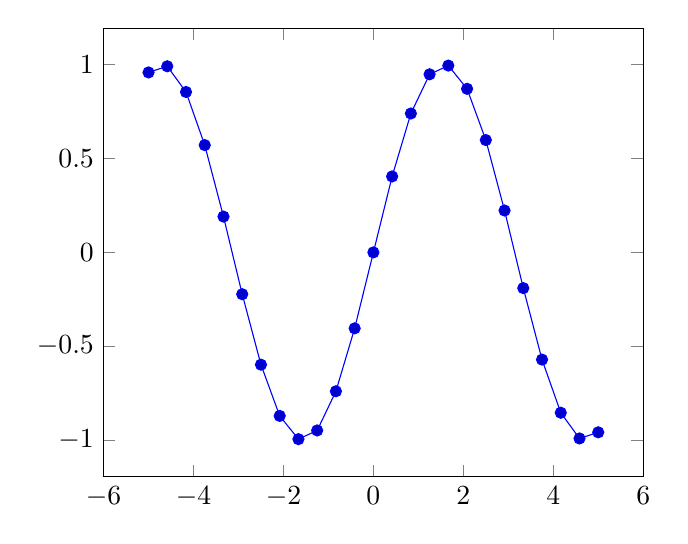
\begin{tikzpicture}
\begin{axis}
\addplot (\x,{sin(\x r)});
\end{axis}
\end{tikzpicture}

\testsubsection{$x^2$}
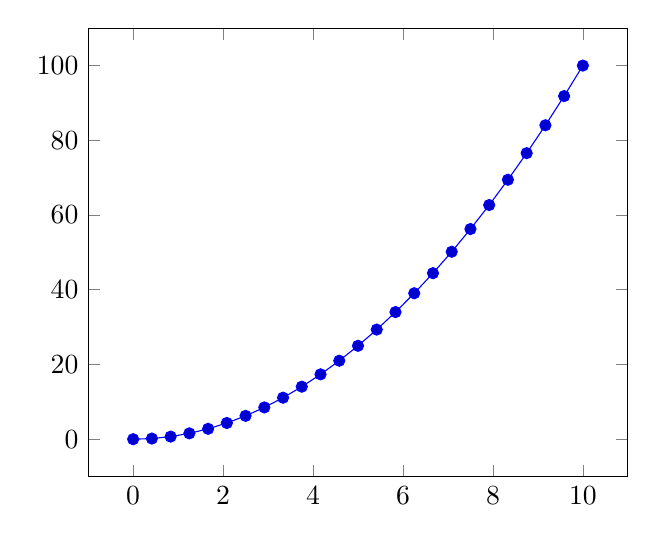
\begin{tikzpicture}
\begin{axis}
\addplot plot[domain=0:10] (\x,\x^2);
\end{axis}
\end{tikzpicture}

% #1: tex expr
% #2: gnuplot expr or empty
% #3: options
\def\testexpression#1#2#3{%
	\testsubsection{$#1$}
	\begin{tikzpicture}
		\begin{axis}[title={$#1$},#3]
			\addplot+[mark=] {#1};
			\def\gnuplotexpr{#2}%
			\ifx\gnuplotexpr\empty
				\def\gnuplotexpr{#1}%
			\fi
			\addplot+[mark=] gnuplot {\gnuplotexpr};
			\legend{\TeX,gnuplot}
		\end{axis}
	\end{tikzpicture}%
}%


\testexpression{x^10}{x**10}{domain=-3:3}

\testexpression{x^10}{x**10}{domain=-3:3000}

\testexpression{x*5*(1-100)/(1-x)}{}{domain=1000:3000}

Das liegt an der relativen genauigkeit und an der enge des datenbereichs:

\testexpression{x*5*(1-100)/(1-x)}{}{samples=500,domain=20:3000}

\testexpression{1/x}{}{domain=1e-10:1e-9,samples=300}

\testexpression
	{exp(0-(x-90)^2 /0.0001)}
	{exp( -(x-90)**2/0.0001)}
	{domain=89.9:90.1,samples=300}

\testexpression{sqrt(abs(x))}{}{domain=-3:3,samples=501}

\testexpression
	{-5+x-x^2 * x/3}
	{-5+x-x**2 * x/3}
	{domain=0:50}

\testexpression
	{-sin(4*deg(x))}
	{-sin(4*x)}
	{domain=0:4*pi,samples=500}

%\tracingmacros=2\tracingcommands=2
\testexpression{max(0,x-4)}{}{samples=300,domain=-2:10}

\testexpression{min(0,x-4)}{}{samples=100,domain=-2:10}

\testexpression{min(0,x-4)}{}{samples=100,domain=-2:10}
